\section{热-质耦合输运的公共模型与离散方法}

本章建立四问共用的连续模型、边界条件、环境驱动与数值方法。各问只在物性关系、终止条件和
求解域三处与本章不同，后续章节只陈述这些差异，不重复整套推导。

\subsection{系统边界与守恒关系}

取药材横截面的径向一维区域 $r\in[0,R]$ 为研究对象，$R$ 在前三问为常数、在问题四随时间变化。
以单位轴向长度的圆环控制体为对象写守恒关系。热量方面，控制体内焓的变化率等于经内外两个
圆柱面净流入的导热量；水分方面，干基含水率的变化率等于净流入的扩散水量。圆柱几何使
两个圆环面的面积不等（内侧面积小、外侧面积大），这一差异在微分形式中表现为 $1/r$ 因子。
按傅里叶导热定律与菲克扩散定律闭合通量\upcite{Tzempelikos2015,Srikiatden2007}，得到

\begin{equation}\label{eq:energy}
\rho(C)\,c_p(C)\,\frac{\partial T}{\partial t}
=\frac{1}{r}\frac{\partial}{\partial r}\!\left(r\,k(C)\,\frac{\partial T}{\partial r}\right),
\end{equation}

\begin{equation}\label{eq:moisture}
\frac{\partial C}{\partial t}
=\frac{1}{r}\frac{\partial}{\partial r}\!\left(r\,D(C,T)\,\frac{\partial C}{\partial r}\right).
\end{equation}

式~\eqref{eq:energy} 中 $T(r,t)$ 为药材内部温度，$\rho$、$c_p$、$k$ 分别为密度、比热容与
导热系数；式~\eqref{eq:moisture} 中 $C(r,t)$ 为干基含水率，$D$ 为水分有效扩散系数。
本文依据题给经验扩散关系，将干基含水率 $C$ 作为有效扩散变量，建立 Fick 型有效扩散模型；
该形式与以湿基质量分数为变量的写法不同，后者会额外引入密度的时间导数，但不声称在一般收缩介质中天然等价于严格局部质量守恒。
两式的系数都可能依赖 $C$ 与 $T$，因此这是一组非线性抛物型方程，
其耦合强度完全由所用物性关系决定。

\subsection{边界条件与初始条件}

药材表面与热空气之间既有对流换热又有对流传质，两者都属第三类边界：表面通量与
药材表面值和空气侧值之差成正比。表面处

\begin{equation}\label{eq:bc_surface}
\left.-k(C)\frac{\partial T}{\partial r}\right|_{r=R}=h\,\bigl[T(R,t)-T_{\rm air}(t)\bigr],\qquad
\left.-D(C,T)\frac{\partial C}{\partial r}\right|_{r=R}=h_m\,\bigl[C(R,t)-C_{\rm air}(t)\bigr],
\end{equation}

其中 $h=25$~W/(m$^2\cdot$K)、$h_m=8\times10^{-7}$~m/s 为题给的对流换热与对流传质系数。
按第三类边界建模而不用第一类，理由见问题一的分析\upcite{Tzempelikos2015,Pereira2014}。
轴心处由几何对称性给出零通量条件

\begin{equation}\label{eq:bc_center}
\left.\frac{\partial T}{\partial r}\right|_{r=0}=0,\qquad
\left.\frac{\partial C}{\partial r}\right|_{r=0}=0 .
\end{equation}

式~\eqref{eq:bc_center} 并非附加假设，而是径向对称场在轴心可微的必然结果。初始时刻药材
温度与含水率均匀

\begin{equation}\label{eq:ic}
T(r,0)=T_0=28~^\circ\mathrm{C},\qquad C(r,0)=C_0=2.55~\mathrm{kg/kg},\qquad R(0)=R_0=2~\mathrm{cm}.
\end{equation}

\subsection{环境驱动的处理}

式~\eqref{eq:bc_surface} 中的 $T_{\rm air}(t)$ 与 $C_{\rm air}(t)$ 来自附件 1 的实测时序，
全部 $241$ 个采样点按分段线性插值，不作两点线性化。附件 1 仅覆盖前 $4$~h，
其后按平台末值保持 $T_{\rm air}=50.0000~^\circ$C、$C_{\rm air}=0.0500$~kg/kg；
$50.165~^\circ$C 与 $0.04986$~kg/kg 仅为末采样点。实测段与外推段的衔接见图~\ref{fig:input_chamber}。

\begin{figure}[H]
  \centering
  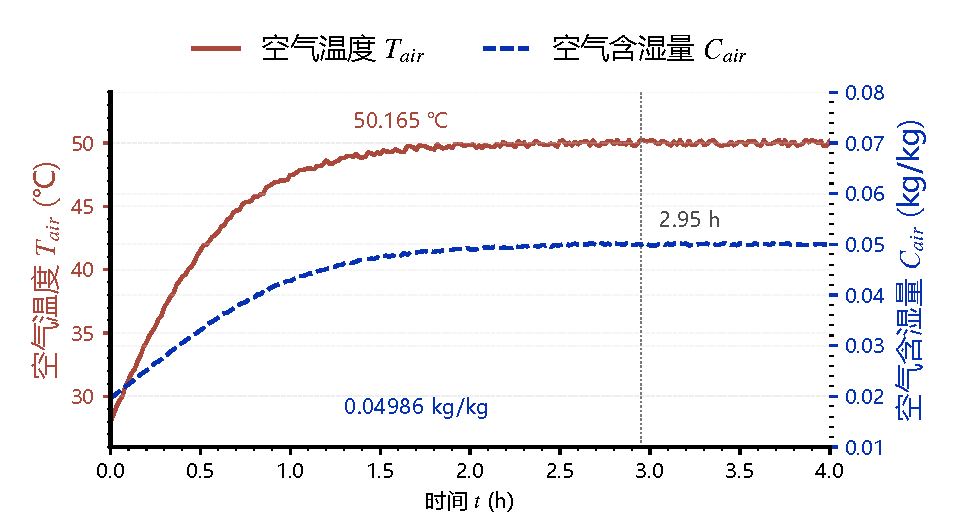
\includegraphics[width=0.76\textwidth,height=0.32\textheight,keepaspectratio]{../figures/fig_input_chamber.pdf}
  \caption{附件 1 干燥室工况的双轴时程}
  \label{fig:input_chamber}
\end{figure}

进入平台后，长时程求解的边界驱动不再随环境变化，内部扩散阻力成为继续失水的限制因素。

\subsection{物性关系与由此决定的数学类型}

三个附录给出三套物性关系，分别用于问题一、问题二至三、问题四。记湿基水分分率
$w=C/(C+1)$、绝对温度 $T_K=T+273.15$。问题一采用常物性

\begin{equation}\label{eq:prop_app2}
\rho=820,\qquad c_p=2600,\qquad k=0.36,\qquad D(C)=7\times10^{-9}\,\mathrm{e}^{-0.89/C},
\end{equation}

问题二与问题三采用

\begin{equation}\label{eq:prop_app3}
\begin{gathered}
\rho=650+128C,\quad c_p=1450+2736w,\quad k=0.21+0.38w,\\
D=2.4\times10^{-3}\,\mathrm{e}^{-0.45/C}\,\mathrm{e}^{-3850/T_K},
\end{gathered}
\end{equation}

问题四采用

\begin{equation}\label{eq:prop_app4}
\begin{gathered}
\rho=760+90C,\quad c_p=1850+2150w,\quad k=0.12+0.20w,\\
D=4.2\times10^{-4}\,\mathrm{e}^{-0.30/C}\,\mathrm{e}^{-3850/T_K}.
\end{gathered}
\end{equation}

三式中扩散系数的指数因子 $\mathrm{e}^{-a/C}$ 表示含水率越低、水分迁移越困难，
$\mathrm{e}^{-3850/T_K}$ 是典型的活化能形式，表示升温促进扩散\upcite{Sander1998}。
指数中的温度必须取绝对温度：若误用摄氏读数，在 $28~^\circ$C 附近该因子会相差十余个数量级。

式~\eqref{eq:prop_app2} 与后两式的区别决定了问题的数学类型。常物性下
式~\eqref{eq:energy} 的系数与 $C$ 无关，且 $D$ 不含温度。在问题一的物性关系下，温度方程与水分方程
完全解耦：温度场可独立求解，水分场仅通过 $D(C)$ 与自身含水率发生非线性关联，无需调用温度场结果。式~\eqref{eq:prop_app3} 与
式~\eqref{eq:prop_app4} 下两条依赖同时接通，两场必须联立推进。
后两套扩散系数在工作区间上的分布见图~\ref{fig:property_maps}。

在 $C\in[0.15,2.55]$、$T\in[28,50]~^\circ$C 上，附录 3 的扩散系数覆盖
$3.35\times10^{-10}$--$1.35\times10^{-8}$~m$^2$/s，附录 4 覆盖
$1.59\times10^{-10}$--$2.50\times10^{-9}$~m$^2$/s，比值介于 $0.186$--$0.476$。
附录 4 的迁移能力系统性地低于附录 3，最多低约五倍：若只换物性而不引入收缩，时长必然显著延长。

\subsection{有限体积离散}

式~\eqref{eq:energy} 与式~\eqref{eq:moisture} 的系数随解变化，不存在通用的解析解，
须数值求解。本文采用有限体积法而非有限差分：有限体积法从控制体积分形式出发，
相邻控制体共用界面通量，离散层面自动满足守恒，圆柱几何的 $1/r$ 因子由界面面积
$2\pi r_{i\pm1/2}$ 自然承担，不需要额外处理奇点\upcite{Patankar2018,Mignone2014}。
这一性质在本题尤其重要，因为烘干时长由累积失水量决定，守恒误差会直接积累成时长误差。

将 $[0,R]$ 等分为 $N$ 个径向区间，设置 $N+1$ 个节点 $r_i$（$i=0,\ldots,N$），并以节点为中心
构造有限体积控制体；轴心与表面采用半宽控制体。三类控制体的单位长度体积分别为

\begin{equation}\label{eq:cv}
V_0=\pi\left(\frac{\Delta r}{2}\right)^{2},\quad
V_i=2\pi r_i\,\Delta r\ (1\le i\le N-1),\quad
V_N=\pi\left(R-r_{N-1/2}\right)\left(R+r_{N-1/2}\right).
\end{equation}

式~\eqref{eq:cv} 的三种写法互不相同：轴心控制体是实心小圆盘，内部控制体含向心汇聚因子
$r_i$，表面控制体是半宽圆环。若照搬直角坐标下的等体积划分，中心区域的体积会被系统性高估，
从而低估中心的升温与失水速率。三类控制体在柱截面上的实际几何见图~\ref{fig:cylinder_cv}。

\begin{figure}[H]
  \centering
  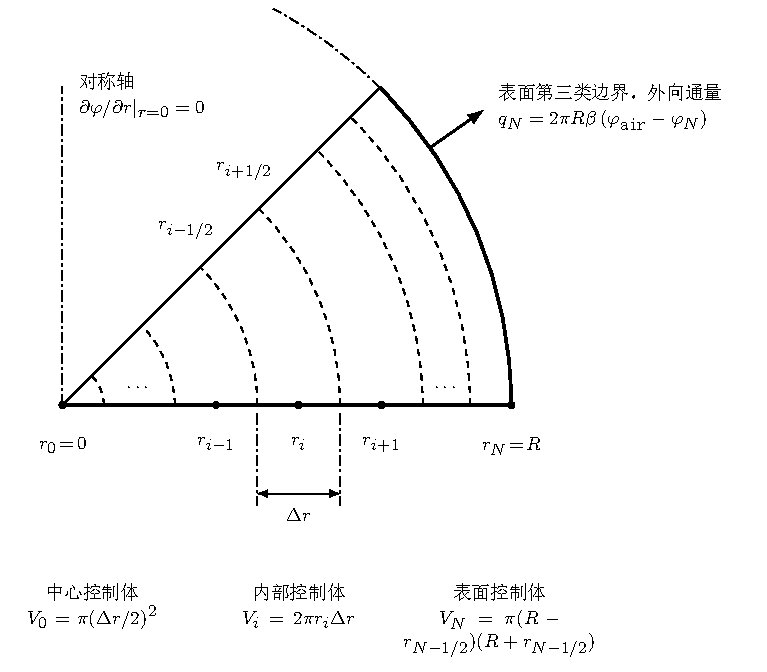
\includegraphics[width=0.60\textwidth,height=0.42\textheight,keepaspectratio]{../figures/tikz_cylinder_cv.pdf}
  \caption{圆柱径向有限体积的控制体划分}
  \label{fig:cylinder_cv}
\end{figure}

图中虚线弧为控制体界面、实心圆点为结点。表面控制体的外向通量由第三类边界
$q_N=2\pi R\,\beta\,(\varphi_{\rm air}-\varphi_N)$ 给出，其中 $\varphi$ 泛指 $T$ 或 $C$、
$\beta$ 泛指 $h/(\rho c_p)$ 或 $h_m$；轴心控制体则由式~\eqref{eq:bc_center} 的
对称条件关闭，不需要虚拟结点。

\subsection{时间推进、界面物性与耦合处理}

时间方向采用全隐式后向 Euler 格式。对通用标量 $\varphi$，在控制体 $i$ 上积分后得到

\begin{equation}\label{eq:implicit_fv}
V_i\,\frac{\varphi_i^{n+1}-\varphi_i^{n}}{\Delta t}
=2\pi r_{i+1/2}\,\Gamma_{i+1/2}\frac{\varphi_{i+1}^{n+1}-\varphi_i^{n+1}}{\Delta r}
-2\pi r_{i-1/2}\,\Gamma_{i-1/2}\frac{\varphi_i^{n+1}-\varphi_{i-1}^{n+1}}{\Delta r},
\end{equation}

其中 $\Gamma$ 为对应的输运系数。显式格式受 $\Delta t\le\Delta r^2/(2\alpha)$ 限制，
本题热扩散率量级下上限约 $0.7$~s，数十小时积分不可行，故对每次冻结系数后的扩散子问题采用后向 Euler 全隐式离散；该子问题无条件稳定，整体非线性耦合的收敛性由随后的 Picard 迭代判据控制。
离散后形成三对角方程组，用 Thomas 算法以 $O(N)$ 求解\upcite{DallOsso2004}。
界面系数取算术平均 $\Gamma_{i+1/2}=\tfrac12(\Gamma_i+\Gamma_{i+1})$；
装配系数满足 $a_i,c_i\le 0$ 且 $b_i>|a_i|+|c_i|$，离散矩阵具有对角占优结构；正式计算未出现非物理振荡，所得温度和含水率剖面保持预期的径向分布特征。

两个场的耦合按固定次序的算子分裂处理。一个时间步内依次完成：
（1）由旧层的 $(C^n,T^n)$ 计算 $\rho$、$c_p$、$k$；
（2）隐式求解温度得 $T^{n+1}$；
（3）由 $(C^n,T^{n+1})$ 计算扩散系数；
（4）隐式求解含水率得 $C^{n+1}$；
（5）对新含水率场施加下界以防非物理负值。
这一次序不可交换：若在求解温度之前计算扩散系数，该系数就退化为由旧温度决定，
温度对传质的促进作用被人为削弱。
随后以 Picard 迭代复核——用新层场重算物性并重解，直至相邻两次迭代的场变化按绝对值
低于 $10^{-6}~^\circ$C（温度）与 $10^{-8}$~kg/kg（含水率）——
以消除分裂本身引入的滞后\upcite{HundsdorferVerwer}。
终止判据只在 Picard 收敛之后检查，避免用尚未收敛的中间场触发停机判定。
四问的实际计算中 Picard 迭代最多 $3$ 次即达到上述收敛标准，说明所选时间步长下分裂误差很小；
下界截断在四问中均未被触发，即含水率场自始至终保持为正。

交付计算按各问取正式配置：问题一为 $N=160$、$\Delta t=0.125$~s，
问题二与问题三为同一次 $N=2560$、$\Delta t=0.25$~s 连续积分，问题四为 $N=1280$、$\Delta t=0.25$~s。
这一组网格与步长的选取依据是收敛性检验，具体证据在数值可信度一章给出。
